% Author:: Sebastien Badia (<seb@sebian.fr>)
% Date:: 2014-04-02 01:36:20 +0200
% vi: set ft=tex :

\section{Technical overview}
\begin{frame}{Outline}
    \tableofcontents[currentsection,hideallsubsections]
\end{frame}

\subsection{OpenStack IaaS}
\begin{frame}{OpenStack IaaS}
  \begin{center}
    IaaS component vs. OpenStack component
  \begin{center}
    \medskip
  \end{center}
  \begin{tabular}{lll}
    Compute & \Fleche & Nova \\
    Images & \Fleche & Glance \\
    Identity & \Fleche & Keystone \\
    Storage & \Fleche & Swift (object), Cinder (block) \\
    Networking & \Fleche & Neutron \\
    Dashboard & \Fleche & Horizon \\
    Telemetry & \Fleche & Ceilometer \\
    Orchestration & \Fleche & Heat \\
  \end{tabular}
  \end{center}
\end{frame}

\subsection{Openstack architecture}
\begin{frame}{OpenStack conceptual architecture}
  \begin{center}
    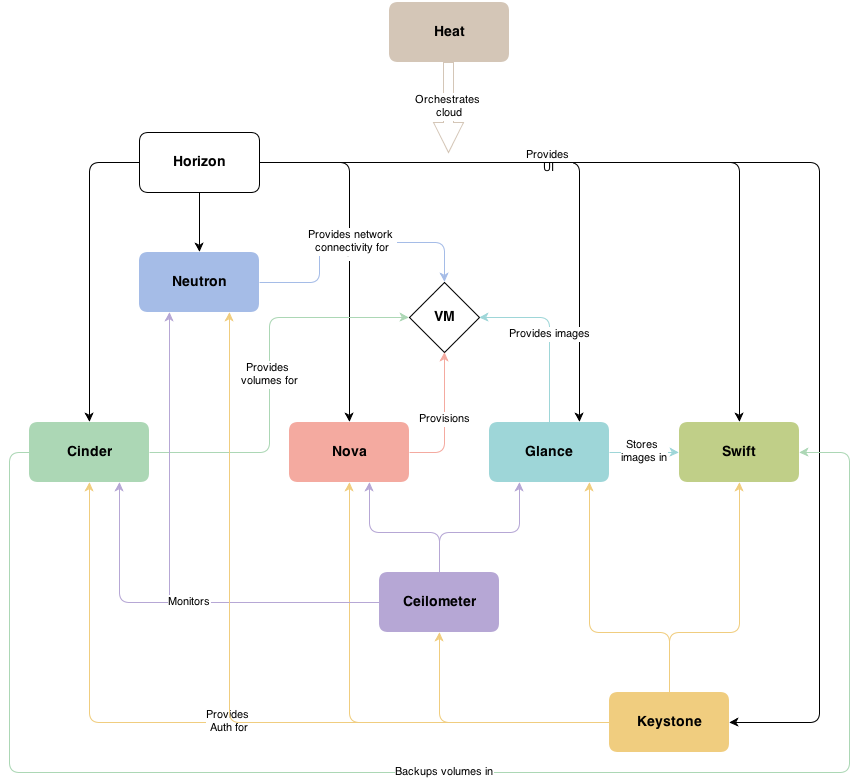
\includegraphics[width=22em]{img/openstack_havana_conceptual_arch}
  \end{center}
\end{frame}

\begin{frame}{OpenStack logical infrastructure}
  \begin{center}
    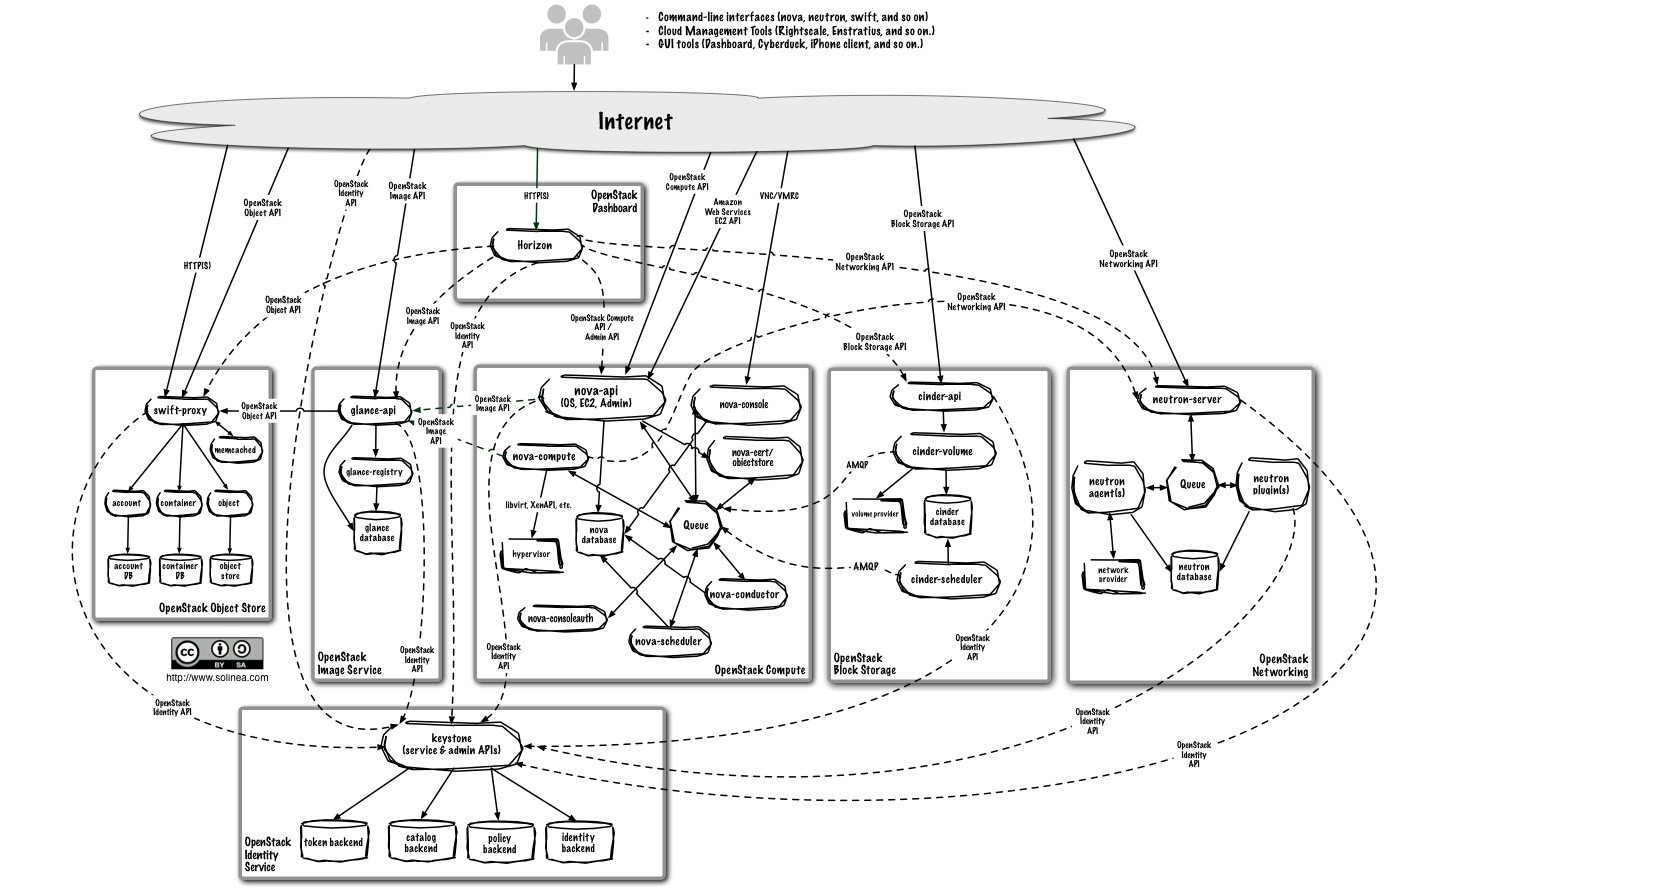
\includegraphics[width=38em]{img/openstack-arch-havana-logical-v1}
  \end{center}
\end{frame}

\subsection{Openstack Compute}
\begin{frame}{OpenStack Compute (\textsl{Nova})}
  \begin{textblock}{}(11,-2)
    
\includegraphics[width=7em]{img/compute}
  \end{textblock}
  \begin{itemize}
    \item Provision and manage virtual machines
      \medskip
    \item Hypervisor support: \textbf{XEN}/XCP, \textbf{KVM}, QEMU, LXC, ESX, ESXi\footnote{\url{http://wiki.openstack.org/HypervisorSupportMatrix}}
      \medskip
    \item OpenStack API (Compute API, Rackspace Cloud Server API)
      \medskip
    \item Support \textbf{live migration} (need a shared storage for instances) (\textsl{Ceph}, \textsl{Swift}, \textsl{NFS\footnote{\tiny{\url{http://docs.openstack.org/trunk/openstack-compute/admin/content/configuring-live-migrations.html}}}, GlusterFS\footnote{\tiny{\url{http://gluster.org/community/documentation/index.php/OSConnect}}}})
      \medskip
    \item Bare-metal, Cells
  \end{itemize}
\end{frame}
\begin{frame}{Nova Scheduler}
  \begin{textblock}{}(12,-2)
    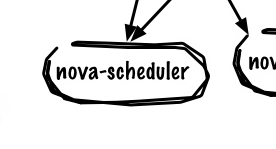
\includegraphics[width=7em]{img/nova-scheduler}
  \end{textblock}
  Nova-scheduler implements a few basic scheduling algorithms
  \begin{itemize}
    \item \textbf{Simple}: hosts whose \textbf{load is least} are chosen to run the instance. The load information may be fetched from a load balancer
    \item \textbf{Chance}: a compute host is chosen \textbf{randomly} across \textbf{availability zones}
    \item \textbf{Zone}: Similar to chance, but the compute host is chosen \textbf{randomly} from within a \textbf{specified zone}
  \end{itemize}
  \center
  \footnotesize
  \begin{tikzpicture}[node distance=1.2em]
  \tikzstyle{every task} = [thick,fill=white]
  \tikzstyle{every sequence} = [thick]
  \tikzstyle{every gateway} = [thick,fill=white]
  \tikzstyle{every event} = [thick,fill=white]
  \tikzstyle{end event} = [event,line width=2.5pt,fill=white]
    \node[event] (start) {};
    \node[task,right=of start] (rpc) {Rpc};
      \draw[sequence,->] (start) -- (rpc);
    \node[task,right=of rpc] (manager) {Scheduler manager};
      \draw[sequence,->] (rpc) -- (manager);
    \node[task,right=of manager] (multi) {Multi Scheduler};
      \draw[sequence,->] (manager) -- (multi);
    \node[task,right=of multi] (filter) {Filter Scheduler};
      \draw[sequence,->] (multi) -- (filter);
    \node[end event,right=of filter] (end) {};
      \draw[sequence,->] (filter) -- (end);
  \end{tikzpicture}
  \begin{itemize}
    \item Compute scheduler support \textttc{filtering} and \textttc{wheighting} to make informed decisions \footnote{\url{http://ibm.co/LUvm2n}}
    \item nova.scheduler.filters (core,compute,ram,cidr,different/same host) \footnote{\url{http://nova.openstack.org/devref/filter\_scheduler.html}}
  \end{itemize}
% shortURL: https://www.ibm.com/developerworks/mydeveloperworks/blogs/e93514d3-c4f0-4aa0-8844-497f370090f5/entry/openstack_nova_scheduler_and_its_algorithm27
\end{frame}

\begin{frame}{OpenStack Object storage (\textsl{Swift})}
  \begin{textblock}{}(11,7.8)
    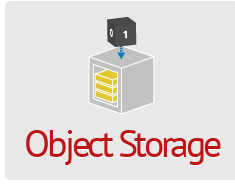
\includegraphics[width=6.5em]{img/swift}
  \end{textblock}
  \begin{itemize}
    \item Object storage (Swift): Redundant (Object/DB)\footnote{\url{http://swift.openstack.org/overview\_replication.html}} and scalable
      \medskip
    \begin{itemize}
      \item Storage via an API (\textbf{not a FS})
        \medskip
      \item \textbf{Long-term} storage system for \textbf{large amounts} of data
        \medskip
      \item Storage abstraction (Ring concept \footnote{\url{http://swift.openstack.org/overview\_ring.html}}, zone and weight of storage)
        \medskip
      \item Works with auth \textbf{token and HTTP API (RESTFull)}
        \medskip
      \item \textbf{Similarity with Amazon S3 (bucket)}
    \end{itemize}
  \end{itemize}
\end{frame}

\begin{frame}{OpenStack Image service (\textsl{Glance})}
  \begin{textblock}{}(11,8)
    
\includegraphics[width=7em]{img/image}
  \end{textblock}
  \begin{itemize}
    \item Image service (Glance): \textbf{Catalog} and \textbf{manage library}\\
      of \textbf{server images}
      \medskip
    \begin{itemize}
      \item Interaction between Nova-compute and Swift or Ceph
        \medskip
        \item Image format
        \begin{itemize}
          \item Conainer (bare,\textbf{ovf},aki,ari,ami)
          \item Disk (raw,vhd,vmdk,vdi,iso,\textbf{qcow2},aki,ari,\textbf{ami})\footnote{http://glance.openstack.org/formats.html}
        \end{itemize}
        \medskip
      \item Manageable by a CLI or an API Rest
        \medskip
      \item \textbf{Image Store} (\textbf{Ceph}, \textbf{Swift}, FS, S3)
        \medskip
      \item Glance support image caching \footnote{http://glance.openstack.org/cache.html}
    \end{itemize}
  \end{itemize}
\end{frame}

\begin{frame}{OpenStack Block storage (\textsl{Cinder})}
  \begin{textblock}{}(11,6)
    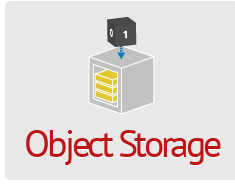
\includegraphics[width=6.5em]{img/swift}
  \end{textblock}
  \begin{itemize}
    \item Enables management of volumes, volume snapshots, and volume types
        \medskip
    \item Support: \textbf{RBD}, \textbf{iSCSI}, Sheepdog, AoE, LeftHand
        \medskip
    \item Similar to Amazon EBS
  \end{itemize}
\end{frame}

\begin{frame}{OpenStack Identity managment (\textsl{Keystone})}
  \begin{textblock}{}(0.3,3)
    
\includegraphics[width=2em]{img/identity-service}
  \end{textblock}
  \begin{itemize}
    \item Provide an \textbf{unified authentication} across \textbf{all openstack projects}
      \medskip
    \item Keystone concepts (\textsl{User managment})
      \medskip
      \begin{itemize}
        \item \textbf{Users}: a human user (login,password,email)
          \medskip
        \item \textbf{Tenants}: a group of users (project or organization)
          \medskip
        \item \textbf{Roles}: determine what operations an user is permitted to perform in a given tenant
          \medskip
      \end{itemize}
    \item Keystone manage also services (services,endpoint,catalog)
      \medskip
    \item OpenStack’s \textbf{Identity API} (XML/JSON API)
      \medskip
    \item Can be backed by LDAP
  \end{itemize}
\end{frame}

\begin{frame}{OpenStack Network (\textsl{Neutron})}
  \begin{itemize}
    \item Provides networking connectivity to VMs
      \medskip
    \item \textbf{Manage network} (L2 and L3) with a Rest API
      \medskip
    \item Networking backend by \textbf{plugins}:
      \medskip
      \begin{itemize}
        \item Open-vSwitch
      \medskip
        \item Linux Bridge
      \medskip
        \item OpenFlow
      \medskip
        \item Floodlight
      \medskip
        \item …
      \end{itemize}
  \end{itemize}
\end{frame}

\begin{frame}{OpenStack Telemetry (\textsl{Ceilometer})}
  \begin{itemize}
    \item Provide \textbf{efficient} collection of \textbf{metering data}, (CPU and network costs)
      \medskip
    \item Custom data by \textbf{plug-ins}.
      \medskip
    \item Produces \textbf{signed} metering messages that cannot be repudiated
  \end{itemize}
\end{frame}

\begin{frame}{OpenStack Orchestration (\textsl{Heat})}
  \begin{itemize}
    \item Provide a \textbf{template-based} for describing a cloud application.
      \medskip
    \item Integrated with \textbf{all} OpenStack ressources
      \medskip
    \item Provide advanced features (\textbf{ha}, \textbf{auto-scaling}, …)
      \medskip
    \item REST API,compatible with AWS CloudFormation
  \end{itemize}
\end{frame}

\begin{frame}{OpenStack Dashboard (\textsl{Horizon})}
  \begin{textblock}{}(12,12.3)
    
\includegraphics[width=1.7em]{img/dashboard}
  \end{textblock}
  \begin{table}[t]
    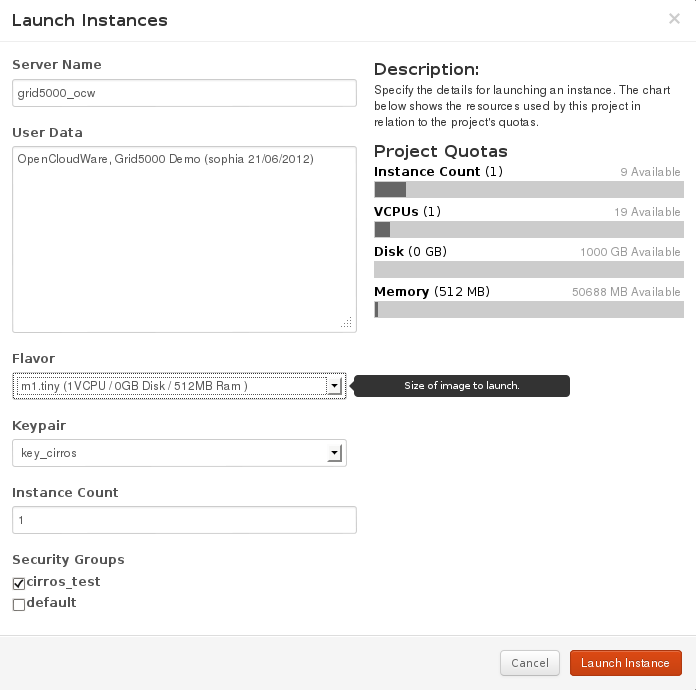
\includegraphics[width=16em]{img/dashboard_ocw}
  \end{table}
    \begin{itemize}
      \item Access and provision \textbf{cloud resources through a web portal}
      \item \textbf{Credentials}, \textbf{users} and \textbf{projects} management
      \item \textbf{Django module} for \textbf{easy} integration/creation
    \end{itemize}
\end{frame}
